\documentclass[resume]{subfiles}


\begin{document}
\section{Systèmes}

\subsection{Mouvement et trajectoire}

\begin{figure}[H]
    \centering
    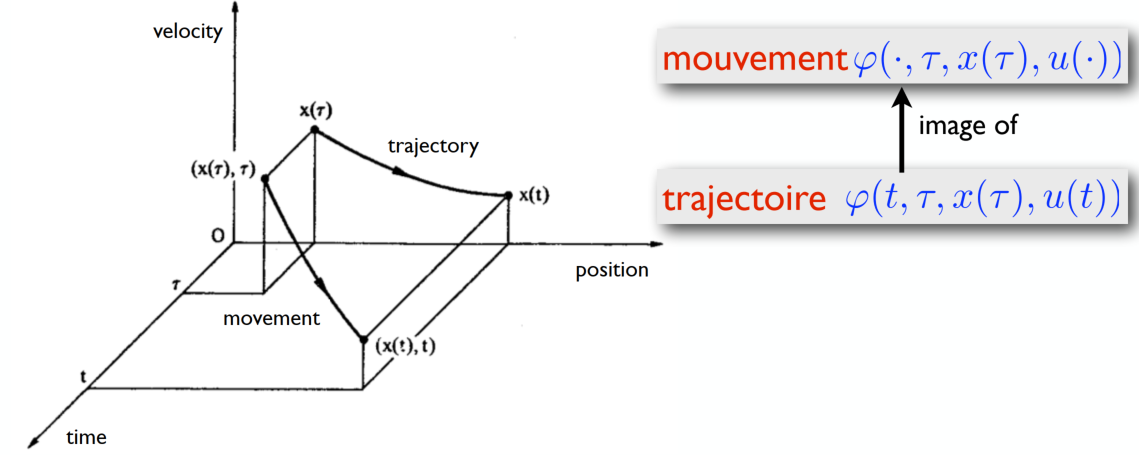
\includegraphics[width=1\columnwidth]{Figures/MouvTraj.png}
\end{figure}

\subsection{Systèmes invariants}

Un système est dit invariant si
\begin{itemize}
\item T est un groupe additif
\item Pour tout $u \in \Omega$ et pour chaque $s \in T$  la fonction $u^s(\cdot)$ obtenue par
  translation ($u(t)=u^s(t+s)$) appartient également à $\Omega$
\item La fonction de translation à la propriété
  $\varphi(t,\tau,x,u(\cdot))=\varphi(t+s,\tau +s,x,u^s(\cdot))$ 
\item La transformation de sortie ne dépend pas explicitement du temps
  $y(t) = \eta(x(t))$ 
\item Si $T=\mathbb{N}$ nous avons un système à temps discret
\item Si $T=\mathbb{R}$ nous avons un système à temps continu  
\end{itemize}

\subsection{Systèmes réguliers}
\begin{itemize}
\item Si les ensembles U, X, et Y sont des espaces vectoriels de
  dimensions finies, le système est dit de dimensions finies
\item Le ‘circuit électrique’ et les ‘2 bacs’ sont deux exemples de
  systèmes de dimensions finies
\item Si une norme est définie pour les espaces vectoriels, il est
  possible de mesurer la distance entre deux éléments et
  d’introduire la notion de régularité  
\end{itemize}

Un système est regulier si
\begin{itemize}
\item $U, X, Y, \Gamma, \Omega$  sont des espaces normés
\item $\varphi$ est continue dans tous ses arguments et $\frac{d\varphi(t,\tau,x,u(\cdot))}{dt}$ est aussi
continue en t partout où u() est continue
\item $\eta$ est continue dans tous ses arguments  
\end{itemize}

Le mouvement d’un système régulier de dimension finie est la solution d’un équation différentielle de la forme: $\frac{dx(t)}{dt}=f(x(t),u(t),t)$ qui satisfait la condition initiale $x(\tau) = x$

Donc un système régulier est représenté par:

\begin{equation}
\begin{cases}
  \dot{x}(t)=f(x(t),u(t),t)\\
   y(t)=g(x(t),t)
\end{cases}
\end{equation}

\subsection{Systèmes linéaires}

Un système est dit linéaire si
\begin{itemize}
\item $U, X, Y, \Gamma, \Omega$  sont des espaces normés
\item $\varphi$ est linéaire en $X \times \Omega$ pour tout $t,\tau\in T$:
\item $\eta$ est linéaire en X pour tout t dans T $\eta(t) = C(t)x(t)$ 
\end{itemize}

Avec un système linéaire. le mouvement peut être
décomposé en la somme des mouvements libre et forcé  

$x(t) = x(\tau) + \int^t_{\tau}\frac{u}{C(\xi)}d\xi = MouvementLibre + MouvementForce$  

\subsection{Système linéaires et réguliers}
\begin{itemize}
\item Si un système de dimensions finies est linéaire et régulier,
  alors son état $x$ satisfait:

  $\frac{dx(t)}{dt} = f(x(t), u(t), t)$ (1)

\item Comme $\varphi$, solution de (1), est linéaire en x et u

  $f(x(t), u(t), t) = A(t)x(t) + B(t)u(t)$ 

\item Alors, un système linéaire est décrit par:
\end{itemize}

\begin{equation}
\begin{cases}
  \dot{x}(t)=A(t)x(t) + B(t)u(t)\\ 
  y(t) = C(t)x(t)
\end{cases}
\end{equation}
\end{document}